% 2D Image with indices
% Author: Peter Steinbach
\documentclass[tikz]{standalone}
%\documentclass[dvisvgm]{standalone}
%\def\pgfsysdriver{pgfsys-tex4ht.def}
\usepackage{units}
\usepackage{tikz}
\usetikzlibrary{calc,math,trees,positioning,arrows.meta,chains,shapes.geometric,shapes.arrows,%
    decorations.pathreplacing,decorations.pathmorphing,shapes,%
    matrix,shapes.symbols,fit,backgrounds}

 \pgfdeclarelayer{back}
 \pgfsetlayers{background,back,main}


\makeatletter
\makeatother

\begin{document}
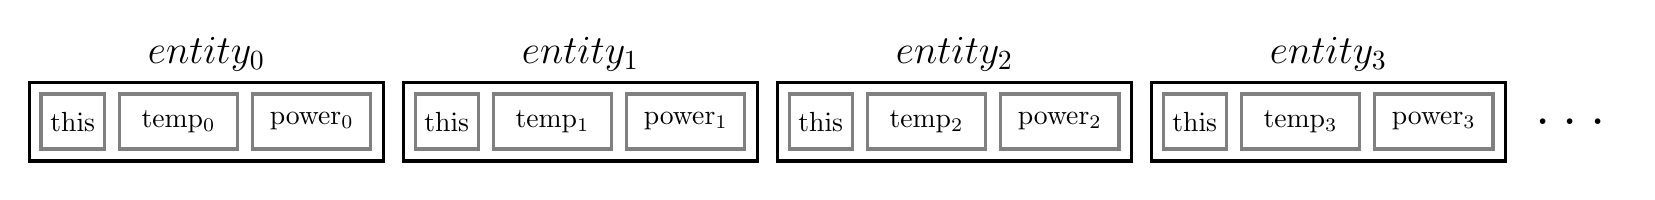
\begin{tikzpicture}

  \node (start) [draw=none] at(0,0) {};
  
  \foreach \i in {0,...,3}
           {
             \node (entity_\i) [rectangle,draw=black,very thick,minimum width=4.5cm,minimum height=1.cm,above] at($(start.east) + (4.75*\i,0)$) {};
             \node (title_\i) [above,font=\Large] at(entity_\i.north) {$entity_\i$};
             \node (thisptr_\i) [rectangle,draw=gray,very thick,anchor=west,minimum height=.7cm,minimum width=.8cm] at($(entity_\i.west)+(.15,0)$) {this};
             \node (temp_\i) [rectangle,draw=gray,very thick,anchor=west,minimum height=.7cm,minimum width=1.5cm] at($(thisptr_\i.east) + (.15,0)$) {temp$_\i$};
             \node (pow_\i) [rectangle,draw=gray,very thick,anchor=west,minimum height=.7cm ,minimum width=1.5cm] at($(temp_\i.east) + (.15,0)$) {power$_\i$};
             }

           \node (dots) [font=\Huge,very thick,right] at($(entity_3.east) + (.2,0)$) {\dots};
  %% \node (start) [draw=none,font=\huge,above] at(0,0) {\textbf{iteration}};
  %% \node (iter_0) [draw=none,font=\huge,above] at($(start.south)+(0,-1.)$) {$0$};
  

  %% \foreach \i in {0,...,15}
  %%  {

  %%    \tikzmath{
  %%      integer \x;
  %%      \x = \i+16;
  %%    }

  %%      \node (mem_\i) [rectangle,draw=gray,very thick,minimum width=1.cm,minimum height=1.cm,anchor=west,font=\Large] at($(iter_0.east)+(1.,0) + (1.1*\i,0)$) {$\i$};
  %%      \node (mem_\x) [rectangle,draw=gray,very thick,minimum width=1.cm,minimum height=1.cm,font=\Large] at($(mem_\i.south) + (0,-.7)$) {$\x$};
     
  %%    }
     
  %%    \node (pref_0) [rectangle,draw=orange,ultra thick,minimum width=9.75cm,minimum height=1.cm,anchor=west] at($(mem_0.west)$) {};
  %%    \node (acc_0) [rectangle,draw=red,ultra thick,minimum width=1.cm,minimum height=1.cm,anchor=west] at($(mem_0.west)$) {};

\end{tikzpicture}
\end{document}
